\documentclass{article}
\usepackage{fancyhdr} % Required for custom headers
\usepackage{lastpage} % Required to determine the last page for the footer
\usepackage{extramarks} % Required for headers and footers
\usepackage{graphicx} % Required to insert images
%\usepackage{lipsum} % Used for inserting dummy 'Lorem ipsum' text into the template
\usepackage{amsmath}
%\usepackage{amsfont}
%\usepackage{amssymb}

\usepackage{multicol}
% Margins
\topmargin=-0.5in
\evensidemargin=0in
\oddsidemargin=-0.5in
\textwidth=7.5in
\textheight=9.0in
\headsep=0.25in 


\pagestyle{fancy}

\rhead{M. Adam} % Top right header
\lhead{Ricotta Cake}
\chead{ }
%\title{}

\begin{document}
%
%PRELIMINARIES:
%
%
%Begin by preheating the oven to 350 $^o$F
%
%\bigskip
%
%\bigskip

\begin{multicols}{2}
Ingredients:
\begin{itemize}
\item 3 eggs
\item 1/2 cup sugar
\item 1 container (16oz.) whole milk ricotta cheese
\item 1/4 cup gluten-free baking mix (must have raising agent)
\item Juice from 1/2 lemon
\item 3-4 gluten-free graham crackers, crushed
\item 2 tbsp of butter for greasing the pie dish
\end{itemize}

\columnbreak

Directions:
\begin{enumerate}
\item Preheat your oven to 325°F.

\item Start off by cracking 3 eggs and place them into a mixing bowl, then add in sugar and mix together. Add the ricotta cheese and blend with the egg and sugar mixture. While it is blending, add in the gluten-free baking mix and continue to blend until it is well incorporated. Finish by adding in fresh lemon juice and blend one more time.

\item Grease your pie dish with butter and sprinkle the graham crackers crumbs evenly over the bottom of the dish. You can crush the graham crackers by using a blender or food processor.

\item Pour the batter over the crumbs and place it in the oven for 25 minutes or until it begins to turn golden brown. Once the cake is golden brown let it cool or place it in the refrigerator so it tastes more like a cheese cake.
\end{enumerate}
\end{multicols}



\begin{center}
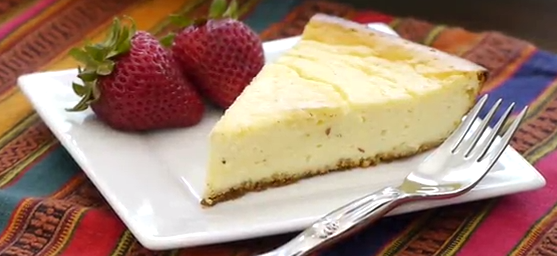
\includegraphics[scale=0.4]{RicottaCake.png}
\end{center}


\end{document} 











